% =====================================================================
% Rozdział 1 – Wstęp (WZÓR, ok. 2 strony)
% Styl bezosobowy. Klucze \cite{} – plik literatura_wzor.bib.
% Rysunek: ../rysunki/para_14_rgb_termowizja.pdf (ścieżki względem folderu praca/).
% Fragmenty oznaczone "% TODO" wymagają sprawdzenia albo decyzji autora.
% =====================================================================

\chapter{Wstęp}
\label{chap:wstep}

\section{Motywacja}
\label{sec:motywacja}

Czerniak jest jednym z najgroźniejszych nowotworów skóry, a jego wczesne wykrycie decyduje o skuteczności leczenia. W ocenie zmian barwnikowych podstawową rolę odgrywa obraz w świetle widzialnym -- zdjęcie kliniczne lub obraz dermatoskopowy -- na którym ocenia się kształt, brzeg i barwę zmiany~\cite{dermoscopy}. Obraz taki nie niesie jednak informacji o procesach fizjologicznych zachodzących w zmianie.

Informację tę może uzupełnić termografia, czyli rejestracja promieniowania podczerwonego emitowanego przez skórę. Skóra zachowuje się niemal jak ciało doskonale czarne o emisyjności 0,96--0,98, dzięki czemu termogram odwzorowuje rozkład temperatury jej powierzchni~\cite{infared-thermal-imaging}. Zmiany nowotworowe mogą różnić się od otoczenia odpowiedzią termiczną, zwłaszcza po kontrolowanym schłodzeniu skóry~\cite{visualization-detection-cancer,magalhaes2019}. Obraz widzialny i obraz termowizyjny mają więc charakter komplementarny: pierwszy zawiera bogatą teksturę, drugi -- informację termiczną, ubogą jednak w szczegóły~\cite{deep-learning}.

Warunkiem wspólnej analizy obu obrazów jest ich rejestracja, czyli sprowadzenie do wspólnego układu współrzędnych. W rozważanym zastosowaniu zadanie to jest trudne z trzech powodów. Po pierwsze, zdjęcie wykonuje się telefonem, a termogram -- osobną kamerą termowizyjną; urządzenia nie są ze sobą sprzężone, różnią się polem widzenia i rozdzielczością (obraz termowizyjny ma 320~$\times$~240 pikseli), a każda para obrazów powstaje z innej odległości i pod innym kątem. Po drugie, intensywności pikseli w obrazie widzialnym i podczerwonym nie są ze sobą bezpośrednio powiązane, przez co zawodzą klasyczne metody oparte na punktach charakterystycznych~\cite{visible-and-infared}; dokładne wyrównanie par obrazów widzialnych i podczerwonych pozostaje problemem otwartym~\cite{deep-learning}. Po trzecie, znamię bez schłodzenia skóry nie jest widoczne na termogramie~\cite{visualization-detection-cancer}, nie może więc samo służyć jako punkt odniesienia (rys.~\ref{fig:para-wstep}).

\begin{figure}[htbp]
  \centering
  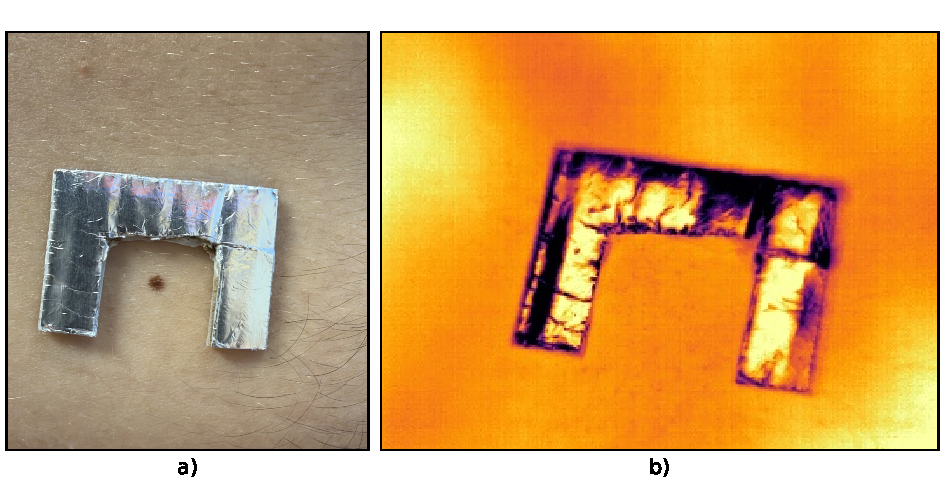
\includegraphics[width=\textwidth]{rysunki/para_14_rgb_termowizja.pdf}
  \caption{Zmiana skórna z naklejonym znacznikiem $\Pi$: a)~zdjęcie wykonane telefonem, b)~obraz termowizyjny 320~$\times$~240 pikseli. Znamię, widoczne na zdjęciu między ramionami znacznika, nie jest widoczne na termogramie. Źródło: opracowanie własne}
  \label{fig:para-wstep}
\end{figure}

Dodatkowym problemem jest weryfikacja wyniku. Nawet poprawnie wyglądające nałożenie obrazów nie gwarantuje, że obszar wyznaczony na zdjęciu odpowiada temu samemu fragmentowi skóry na termogramie. Ręczne oznaczanie punktów kontrolnych w każdej parze obrazów jest pracochłonne, dlatego pożądane jest rozwiązanie, które ocenia zgodność wyznaczenia obszaru automatycznie. Powyższe obserwacje stanowią motywację do podjęcia niniejszej pracy.

\section{Cel i zakres pracy}
\label{sec:cel}

Celem pracy jest opracowanie, implementacja oraz ocena systemu informatycznego umożliwiającego rejestrację i wspólną analizę obrazów dermatologicznych pochodzących z dwóch modalności: zdjęcia RGB wykonanego telefonem oraz obrazu termowizyjnego. System sprowadza oba obrazy do wspólnej przestrzeni odniesienia, przenosi obszar zainteresowania (ang.~\textit{region of interest}, ROI) między modalnościami i wyznacza jego parametry ilościowe. Zgodność wyznaczenia tego samego obszaru w obu modalnościach system weryfikuje, porównując maski segmentacji uzyskane modelami dedykowanymi każdej modalności, a wynikiem jest raport zawierający miary zgodności masek.
% TODO: porównać brzmienie celu z kartą tematu pracy (moja PG).

Aby osiągnąć ten cel, zrealizowano następujące zadania:
\begin{enumerate}
  \item przegląd literatury dotyczącej rejestracji obrazów wielomodalnych, segmentacji obrazów medycznych oraz miar oceny obu procesów;
  \item analizę wymagań i projekt systemu, obejmujący przypadki użycia, architekturę, diagram klas, bazę danych SQLite oraz interfejs użytkownika;
  \item zaprojektowanie znacznika referencyjnego w kształcie litery $\Pi$ (35~$\times$~26~mm, szerokość paska 9~mm, otwór 17~$\times$~17~mm), widocznego w obu modalnościach;
  \item zebranie własnego zbioru danych: 94 par zdjęcie--termogram przedstawiających 34 znamiona, wraz z ręcznymi adnotacjami wykonanymi w programie CVAT;
  \item implementację modułu rejestracji opartego na automatycznej detekcji znacznika i maksymalizacji rozszerzonego współczynnika korelacji (ECC);
  \item przygotowanie modeli segmentacji dla obu modalności: modelu PanDerm z dekoderem UperNet do segmentacji znamienia na zdjęciu oraz sieci U-Net do segmentacji znacznika na obrazie termowizyjnym;
  \item implementację przeniesienia ROI, pomiarów w milimetrach, miar zgodności masek oraz zapisu współrzędnych i surowej intensywności pikseli obrazu termowizyjnego w obszarze znamienia;
  \item implementację aplikacji z interfejsem graficznym, przetwarzania wsadowego i raportowania wyników;
  \item weryfikację systemu, obejmującą ocenę dokładności rejestracji, zgodności masek między modalnościami oraz jakości segmentacji;
  \item przygotowanie dokumentacji technicznej i instrukcji użytkownika.
\end{enumerate}

Zakres pracy nie obejmuje diagnostyki ani klasyfikacji zmian skórnych -- system nie stanowi narzędzia diagnostycznego. System zapisuje surowe intensywności pikseli obrazu termowizyjnego w obszarze znamienia, ale nie przelicza ich na temperaturę ani ich nie interpretuje; termografia dynamiczna stanowi jedynie kontekst rozważań.
Ponieważ znamię nie jest widoczne na termogramie, obszarem porównywanym między modalnościami jest otwór znacznika referencyjnego, w którym znajduje się znamię. Badania przeprowadzono na danych zebranych jednym zestawem urządzeń.

Wkład własny autora obejmuje projekt znacznika, zebranie i opisanie zbioru danych, metodę rejestracji opartą na maskach znacznika, douczenie i trening modeli segmentacji, badania weryfikacyjne oraz implementację aplikacji i bazy danych. W pracy wykorzystano gotowy koder modelu PanDerm udostępniony przez jego autorów~\cite{yan2025panderm} oraz biblioteki programistyczne wymienione w rozdziale~\ref{chap:projekt}.

\section{Struktura pracy}
\label{sec:struktura}

Praca składa się z siedmiu rozdziałów oraz dwóch dodatków. W rozdziale~\ref{chap:stan-wiedzy} przedstawiono przegląd literatury dotyczącej obrazowania zmian skórnych, rejestracji obrazów wielomodalnych, segmentacji oraz miar oceny. Rozdział~\ref{chap:analiza} zawiera analizę projektową: założenia, wymagania, przypadki użycia i architekturę systemu. W rozdziale~\ref{chap:projekt} opisano projekt systemu, w tym dobór technologii, projekt znacznika referencyjnego, bazy danych, diagram klas i interfejs użytkownika. Rozdział~\ref{chap:implementacja} przedstawia implementację poszczególnych modułów, a rozdział~\ref{chap:testy} -- wyniki badań weryfikacyjnych. Pracę zamyka podsumowanie wraz z kierunkami dalszych prac. Dodatek~A zawiera instrukcję użytkownika, a Dodatek~B -- dokumentację techniczną.
